\mychapter{6}{Base de datos empleada}

La base de datos empleada ha sido una de las bases de datos más utilizadas y trabajadas para el estudio del Alzheimer, que es la base de datos conocida como \textbf{ADNI (Alzheimer’s Disease Neuroimaging Initiative)}. La base de datos pone a disposición datos clínicos de pacientes tales como: imágenes MRI y PET, informes genéticos, test cognitivos y biomarcadores de la sangre. Estos pacientes pertenecen a un grupo de estudio voluntario realizado en Norte América dentro de los cuales se incluye pacientes que padecen de Alzheimer, pacientes que muestran un deterioro cognitivo leve y grupos de control, es decir, sujetos sanos.\\

El estudio de ADNI ha tenido tres fases: ADNI1, ADNI GO y ADNI2. En cada una de ellas se incorporaban pacientes nuevos para su evaluación médica. Esta evaluación y seguimiento médico se usaban para detectar cualquier patología de Alzheimer en los pacientes.\\

En nuestro caso se ha utilizado un subconjunto dentro de ADNI en el cuál se había realizado cierto post-procesamiento de las imágenes obtenidas que será explicado a continuación.\\
\section{Post procesamiento}

El post-procesamiento está compuesto por los siguientes pasos:
\begin{itemize}
	\item \textbf{\textit{Spatially Normalized}:} Con este paso lo que se consigue es que un mismo pixel corresponda a la misma posición en dos imágenes cerebrales distintas.
	\item \textbf{\textit{Masked}:} Con este paso conseguimos aislar la masa cerebral eliminando el cráneo. 
	\item \textbf{\textit{N3 Correction}:} Con este paso realizamos una corrección de la intensidad en la imagen.
\end{itemize}
\label{postproces}

Esto permite que tengamos unas imágenes escaladas, centradas y con solo la masa cerebral, lo que nos puede ayudar a que la red aprenda mejores filtros para realizar la clasificación de las imágenes.\\
\begin{figure}[H]
	\centering
	\caption{Ejemplo de una imagen con el post-procesamiento relatado en \ref{postproces}}
	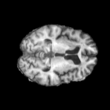
\includegraphics[height=300px,width=300px]{./imagenes/ejemplo_imagen.png}
\end{figure}

\section{Software de visualización de las imágenes}

Para la visualización de estas imágenes podemos hacer uso de varias herramientas. La utilizada para la visualización de las imágenes en formato \textit{NIFTI} ha sido el software \textbf{MRIcron}\cite{mricron}. Este software nos permite visualizar los diferentes cortes cerebrales (coronal, sagital y axial) que están contenidos en el archivo NIFTI.\\

\begin{figure}[H]
	\centering
	\caption{Ejemplo de visualización de una imagen con el software MRIcron \cite{mricron}}
	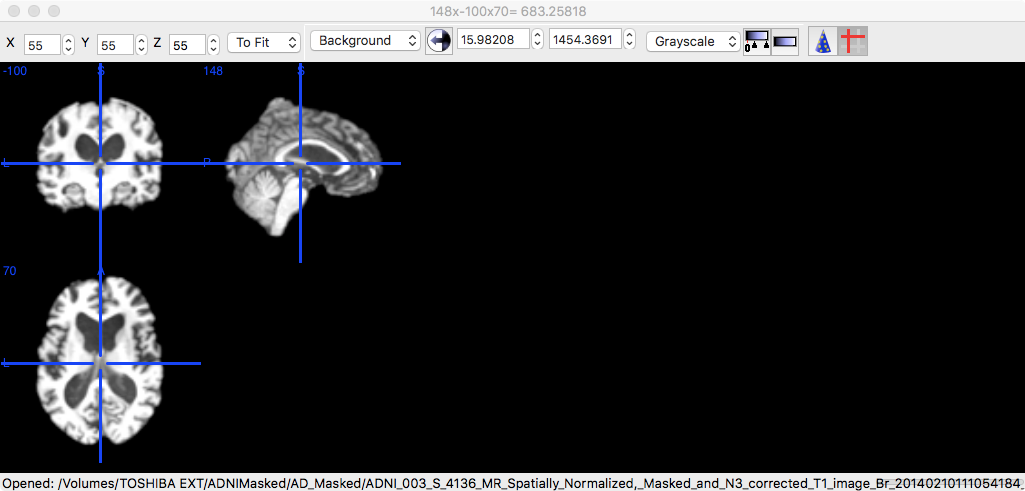
\includegraphics[width=\textwidth]{./imagenes/ejemplomricron.png}
\end{figure}

\section{Separación de las imágenes por tipos}

En cuanto a la clasificación de las imágenes, anteriormente cada imagen tenía asociado un archivo \textit{XML} donde venía resumida la información del paciente y a qué tipo de grupo pertenecía. Pero durante este año se ha llevado a cabo una reorganización de la base de datos por lo que ahora, para la separación de los pacientes según el tipo, se utiliza la búsqueda avanzada señalando en una casilla que tipo de pacientes quieres buscar. Así también se han obtenido los imágenes de los pacientes a las que se le había aplicado el post-procesamiento previamente explicado.